\section{Методы решения задач линейной алгебры}

\subsection{Постановка задачи}
1.1 Реализовать алгоритм LU -  разложения матриц (с выбором главного элемента) в виде программы. Используя разработанное программное обеспечение, решить систему линейных алгебраических уравнений (СЛАУ). Для матрицы СЛАУ вычислить определитель и обратную матрицу.

{\bfseries Вариант:} 19
\begin{equation}
        \left\{ 
        \begin{array}{ll} 
        -8x_1 + 5x_2 + 8x_3 -6x_4 = -144 \\
        2x_1 + 7x_2 - 8x_3 - x_4 = 25\\
        -5x_1 - 4x_2 + x_3 - 6x_4 = -21\\
        5x_1 - 9x_2 - 2x_3 + 8x_4 = 103\\
        \end{array}\right.
\end{equation}
\pagebreak

\subsection{Результаты работы}

\begin{figure}[h!]
\centering
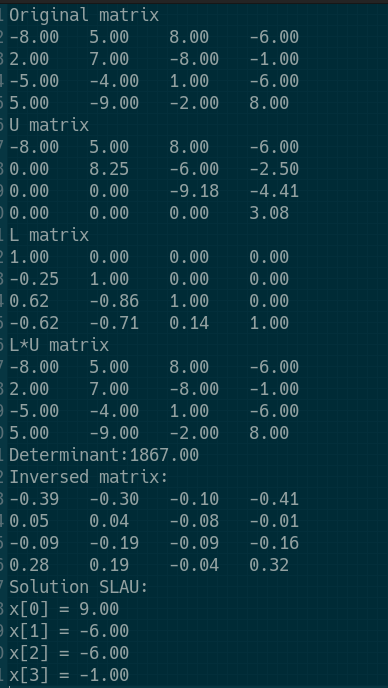
\includegraphics[width=.5\textwidth]{lab1.1}
\caption{Вывод в консоли}
\end{figure}
\pagebreak

\vfill

\subsection{Исходный код}

\lstinputlisting[title=\texttt{Lab1.1.cpp}]{../stud/saifullin/task1.1/Lab1.1.cpp}
\pagebreak
